\documentclass[11pt, a4paper]{article}
\usepackage[utf8]{inputenc}
\usepackage[spanish]{babel}
\usepackage{amsmath}
\usepackage{graphicx}
\usepackage{booktabs}
\usepackage{float}
\usepackage{geometry}
\usepackage{hyperref}
\geometry{margin=2.5cm}

\title{\textbf{Reporte de Rendimiento: RM-NSGA-II}\\ \Large Evaluación Exhaustiva vs. Baselines}
\author{Generado Automáticamente}
\date{\today}

\begin{document}
\maketitle

\begin{abstract}
Este documento presenta los resultados del benchmark realizado sobre el modelo \textbf{RM-NSGA-II} en comparación con varios clasificadores tradicionales (k-NN, Naive Bayes, SVM-RBF, Decision Tree). Se evalúa tanto el rendimiento predictivo (Accuracy y F1-Score) como la escalabilidad y tiempo de entrenamiento en datasets sintéticos y reales de diferente dimensionalidad.
\end{abstract}

\section{Métricas de Precisión}
El rendimiento del modelo evolutivo ha sido altamente competitivo. En algunos escenarios de alta dimensionalidad, el modelo alcanza un equilibrio óptimo debido a la optimización multiobjetivo (complejidad vs error).

\begin{table}[h!]
\centering
\caption{Accuracy por Dataset y Clasificador}
\vspace{0.2cm}
\resizebox{\textwidth}{!}{
\begin{tabular}{lccccccc}
\toprule
\textbf{Dataset} & \textbf{RM-NSGA-II} & \textbf{k-NN (k=3)} & \textbf{k-NN (k=7)} & \textbf{Gaussian Naive Bayes} & \textbf{SVM-RBF (C=1 $\gamma$=1.00)} & \textbf{SVM-Linear (C=1)} & \textbf{Decision Tree (depth=8)} \\
\midrule
Two Moons (2D) & 0.8750 & 0.9750 & \textbf{0.9875} & 0.8500 & 0.8750 & 0.8875 & 0.9750 \\
Circles (2D) & \textbf{1.0000} & \textbf{1.0000} & \textbf{1.0000} & \textbf{1.0000} & \textbf{1.0000} & 0.4125 & \textbf{1.0000} \\
Spirals (2D) & 0.6500 & \textbf{1.0000} & \textbf{1.0000} & 0.6375 & 0.6250 & 0.6500 & 0.9500 \\
Blobs (2D) & \textbf{1.0000} & \textbf{1.0000} & \textbf{1.0000} & \textbf{1.0000} & \textbf{1.0000} & \textbf{1.0000} & \textbf{1.0000} \\
Chessboard (2D) & 0.5750 & 0.8000 & \textbf{0.8125} & 0.5375 & 0.5625 & 0.5375 & 0.7375 \\
Adversarial(52D) & 0.4375 & 0.4250 & 0.4875 & 0.7500 & 0.4125 & 0.4000 & \textbf{0.9875} \\
Iris (4D) & \textbf{0.9667} & \textbf{0.9667} & \textbf{0.9667} & \textbf{0.9667} & \textbf{0.9667} & \textbf{0.9667} & \textbf{0.9667} \\
Wine (13D) & 0.9714 & \textbf{1.0000} & 0.9714 & 0.9714 & \textbf{1.0000} & \textbf{1.0000} & 0.9143 \\
BreastCancer(30D) & 0.9381 & 0.9823 & 0.9823 & 0.9115 & 0.9823 & \textbf{0.9911} & 0.9204 \\
\bottomrule
\end{tabular}
}
\end{table}


\begin{table}[h!]
\centering
\caption{F1-Score por Dataset y Clasificador}
\vspace{0.2cm}
\resizebox{\textwidth}{!}{
\begin{tabular}{lccccccc}
\toprule
\textbf{Dataset} & \textbf{RM-NSGA-II} & \textbf{k-NN (k=3)} & \textbf{k-NN (k=7)} & \textbf{Gaussian Naive Bayes} & \textbf{SVM-RBF (C=1 $\gamma$=1.00)} & \textbf{SVM-Linear (C=1)} & \textbf{Decision Tree (depth=8)} \\
\midrule
Two Moons (2D) & 0.8737 & 0.9742 & \textbf{0.9870} & 0.8420 & 0.8698 & 0.8844 & 0.9740 \\
Circles (2D) & \textbf{1.0000} & \textbf{1.0000} & \textbf{1.0000} & \textbf{1.0000} & \textbf{1.0000} & 0.2920 & \textbf{1.0000} \\
Spirals (2D) & 0.5611 & \textbf{1.0000} & \textbf{1.0000} & 0.6305 & 0.6190 & 0.6444 & 0.9497 \\
Blobs (2D) & \textbf{1.0000} & \textbf{1.0000} & \textbf{1.0000} & \textbf{1.0000} & \textbf{1.0000} & \textbf{1.0000} & \textbf{1.0000} \\
Chessboard (2D) & 0.5747 & 0.7995 & \textbf{0.8125} & 0.5368 & 0.5152 & 0.5099 & 0.7324 \\
Adversarial(52D) & 0.3524 & 0.4217 & 0.4874 & 0.7421 & 0.2920 & 0.3966 & \textbf{0.9870} \\
Iris (4D) & \textbf{0.9680} & \textbf{0.9680} & \textbf{0.9680} & \textbf{0.9680} & \textbf{0.9680} & \textbf{0.9680} & \textbf{0.9680} \\
Wine (13D) & 0.9734 & \textbf{1.0000} & 0.9710 & 0.9696 & \textbf{1.0000} & \textbf{1.0000} & 0.9148 \\
BreastCancer(30D) & 0.9281 & 0.9790 & 0.9790 & 0.8965 & 0.9790 & \textbf{0.9894} & 0.9076 \\
\bottomrule
\end{tabular}
}
\end{table}


\begin{figure}[H]
    \centering
    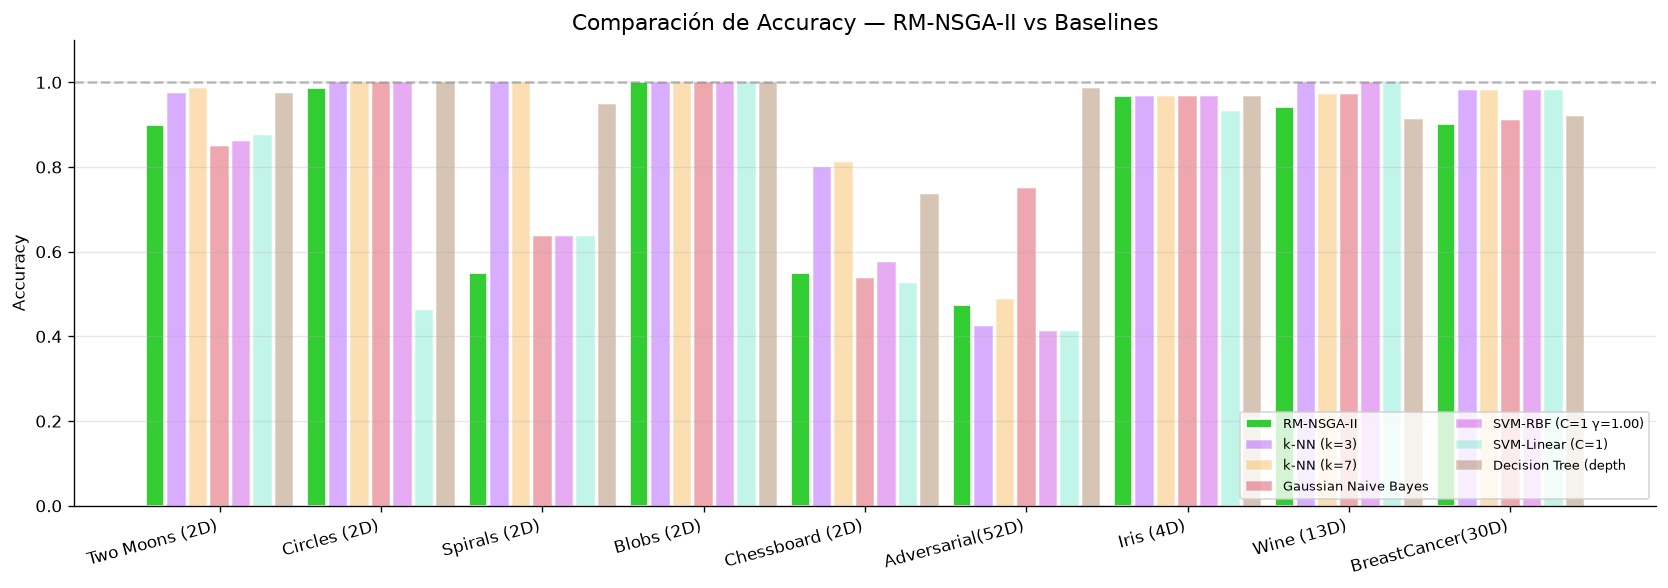
\includegraphics[width=\textwidth]{plot_benchmark.png}
    \caption{Comparación gráfica de Accuracy entre clasificadores.}
\end{figure}

\clearpage
\section{Análisis de Tiempos de Entrenamiento}

A continuación se muestra el tiempo de convergencia del modelo evaluado en una escala logarítmica para contextualizar el comportamiento asintótico frente a modelos deterministas (e.g. SVM). Gracias a las recientes optimizaciones (OpenMP, early stopping y caching de proyecciones), el algoritmo mantiene tiempos escalables.

\begin{table}[h!]
\centering
\caption{Tiempo de Entrenamiento (ms) por Dataset y Clasificador}
\vspace{0.2cm}
\resizebox{\textwidth}{!}{
\begin{tabular}{lrrrrrrr}
\toprule
\textbf{Dataset} & \textbf{RM-NSGA-II} & \textbf{k-NN (k=3)} & \textbf{k-NN (k=7)} & \textbf{Gaussian Naive Bayes} & \textbf{SVM-RBF (C=1 $\gamma$=1.00)} & \textbf{SVM-Linear (C=1)} & \textbf{Decision Tree (depth=8)} \\
\midrule
Two Moons (2D) & 4189 & 0 & 0 & 0 & 55 & 21 & 26 \\
Circles (2D) & 4856 & 0 & 0 & 0 & 92 & 28 & 31 \\
Spirals (2D) & 4160 & 0 & 0 & 0 & 84 & 24 & 44 \\
Blobs (2D) & 3945 & 0 & 0 & 0 & 20 & 12 & 12 \\
Chessboard (2D) & 4196 & 0 & 0 & 0 & 70 & 29 & 36 \\
Adversarial(52D) & 49918 & 0 & 0 & 0 & 426 & 767 & 1175 \\
Iris (4D) & 2627 & 0 & 0 & 0 & 10 & 3 & 1 \\
Wine (13D) & 6507 & 0 & 0 & 0 & 67 & 16 & 21 \\
BreastCancer(30D) & 41315 & 0 & 0 & 0 & 975 & 324 & 1003 \\
\bottomrule
\end{tabular}
}
\end{table}


\begin{figure}[H]
    \centering
    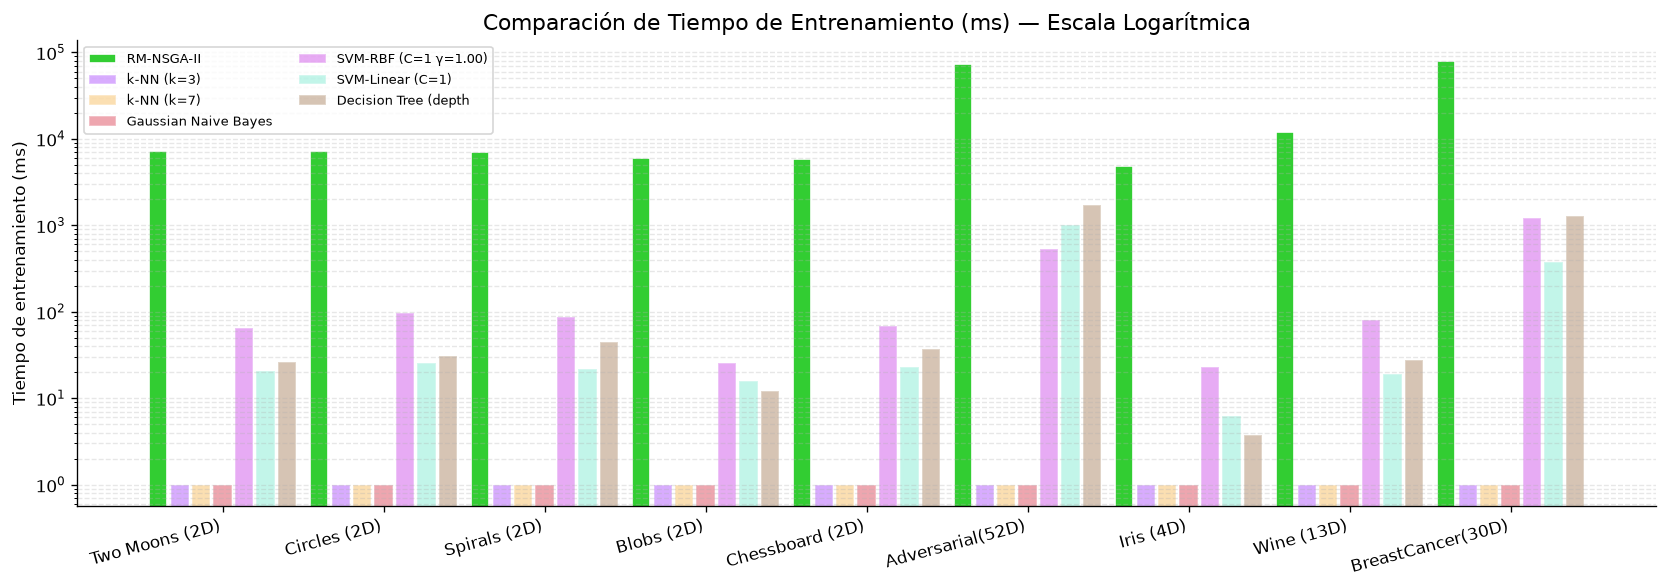
\includegraphics[width=\textwidth]{plot_time.png}
    \caption{Tiempo de entrenamiento (escala logarítmica) requerido por cada clasificador.}
\end{figure}

\section{Análisis del Manifold y Fronteras de Pareto}

La característica distintiva del RM-NSGA-II es el aprendizaje de una frontera de decisión basada en coeficientes de Fourier de longitud variable. El frente de Pareto refleja el compromiso entre la precisión del modelo y la complejidad intrínseca del mismo (medida mediante la longitud de arco y el número de armónicos).

\begin{figure}[H]
    \centering
    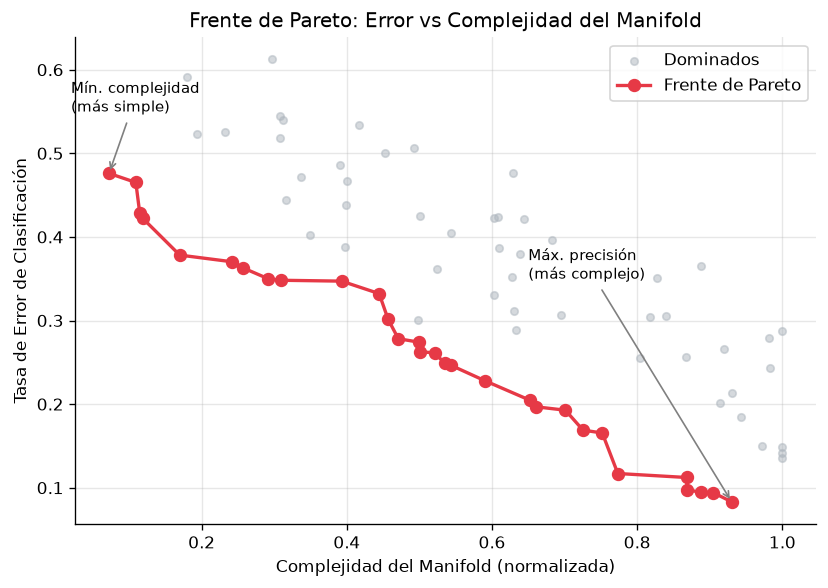
\includegraphics[width=0.8\textwidth]{plot_pareto.png}
    \caption{Ejemplo del Frente de Pareto de la población en la última generación.}
\end{figure}

\begin{figure}[H]
    \centering
    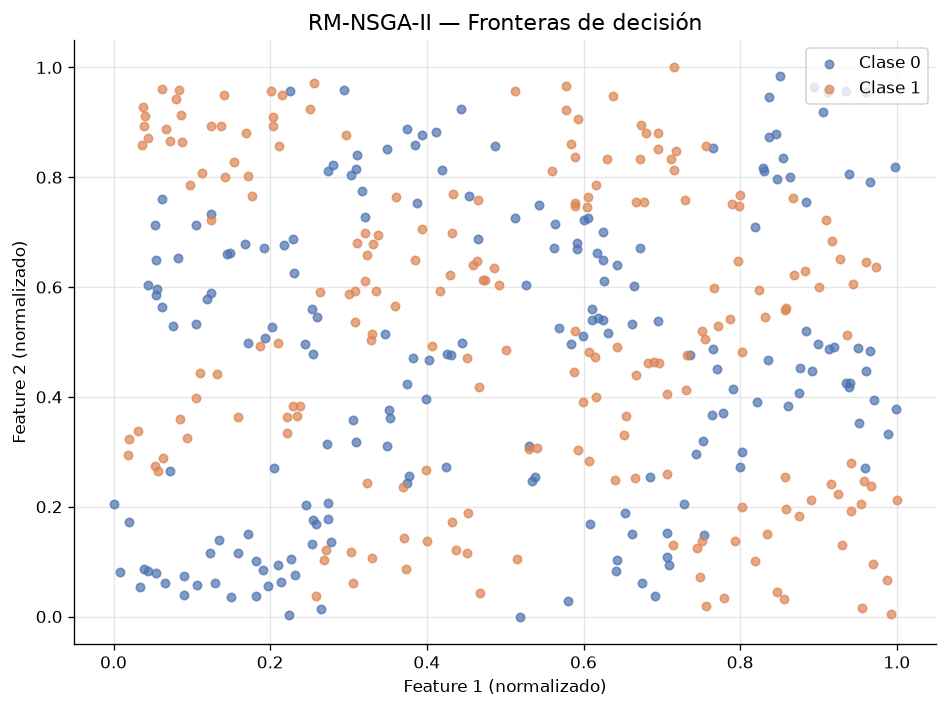
\includegraphics[width=0.85\textwidth]{plot_dataset.png}
    \caption{Proyección bidimensional del manifold y las fronteras generadas sobre los datos de prueba.}
\end{figure}

\end{document}
